% !TEX root = ../report.tex

\clearpage
\chapter{Pattern Documentation}
\label{ch:patterns}
This chapter describes the patterns used in Docker identified by us. We documented the patterns as described by Harrison et al.\cite{usingpatternscapture}, with added information about where the pattern was found (traceability).

\section{Client-Server}

% see https://docs.docker.com/engine/introduction/understanding-docker/

\begin{description}
\item [Traceability]~\\
The Client-Server pattern can be deducted from the online documentation\cite{dockerarchi}.

The Client-Server pattern can be deducted from the `What is Dockers architecture?' section of the online documentation\cite{dockerarchi}.

\item [Source]~\\
Architectural patterns revisited -- a pattern language, P. 29 \cite{avgeriou2005architectural}

\item [Issue]~\\
It should be possible for Docker containers to be controlled remotely and a single interface should be able to control containers on multiple hosts (e.g. in the cloud).

Additionally, certain operating systems lack the underlying technologies necessary for running containers. For those OSes, it should be possible to call remote daemons running on operating systems which are supported. % /WindowsBashing

\item [Solution]~\\
Docker uses a {Client-Server} architecture. The client, a binary supplying a command-line interface, act as the primary interface for the user. The user enters commands into this client, which are then send to a server: the Docker daemon. 


\item [Assumptions/Constraints]~
\begin{itemize}
\item The versions of the client binary and the server binary should match. Different versions can cause problems.
\item All the services offered by the daemon have to be made available to the client using a REST interface.
\end{itemize}
~\\[-1.7cm]
\item [Rationale] ~\\
The daemon is a background process, which supplies the requested services to the client. The daemon exposes a REST interface.

For Docker, the client can be configured to connect to other daemon processes than the one running on the local machine. It can be configured to connect to remote Docker daemons as well, allowing the user to issue commands to daemons running remotely.

%todo move above to architecture chapter 

By separating the client and server it is possible to use the same client to issue commands to different daemons, running on different hosts.
It is also possible to use the client on operating systems that do not support running containers.

\item [Implications]~\\
The use of the {Client-Server} pattern results in two different executable binaries: a daemon and a client. 

The use of the {Client-Server} pattern increases the interoperability, since the client can send commands to daemons running on remote machines and the local machine.

Additionally, the portability is increased, since the client can run on Operating Systems that cannot run containers themselves.


\item [Related Patterns]~\\


\end{description}

\clearpage
\section{Layers}
% see https://www.docker.com/sites/default/files/what-is-vm-diagram.png
Layers pattern is a architectural pattern that consists of several layers, which
each layer provides a set of services to the layer above and uses the services
of the layer below. Docker implements this pattern to separate the concerns of
each component with independent functionalities. Layers pattern implementation
of Docker, based on our investigation, is shown in Figure \ref{fig:layers-pattern}.
% \newglossaryentry{OS}{name=OS, description={Operating System}}

\begin{figure}[H]
\centering
\includegraphics[scale=0.5]{5-patterns/images/LayersPattern.png}
\caption{A layered overview of the Docker.}
\label{fig:layers-pattern}
\end{figure}

\begin{description}
\item [Traceability]~\\
Layers is implicitly mentioned in the Docker architecture in the online
documentation, specifically in the \textit{What is Docker’s architecture?}
section \cite{dockerarchi}.

\item [Source]~\\
Architectural patterns revisited -- a pattern language, P. 29
\cite{avgeriou2005architectural}

\item [Issue]~\\
Docker's features, e.g., hosting the image, creating image, running container,
and daemon supervision, vary in terms of functionality. Single
implementation of those features will certainly result in abundant usage of
resource because hosting the image means there must be huge amount of disk space
available. Overlapping may also occur since multiple Docker instances may have
the same images, which is actually can be stored and organized elsewhere. Docker
also has several dependencies, especially the Linux kernel components
(\texttt{namespaces} and \texttt{cgroups}) for OS level virtualization.
Furthermore, Docker mostly needs remote supervision or control, since usually
Docker is run on the cloud. Therefore, the features must be separated into
several independent components and their dependencies and communication have to
be clearly separated and maintained.

\item [Assumptions/Constraints]~\\
Docker is able to run only in Linux kernel since it makes use of
\texttt{namespaces} and \texttt{cgroups} technology, which is only available in
Linux kernel. However, Docker is also possible to be run on other OS
although using virtual machine. The connection between local and remote
components are carried out through secured TCP/IP connection.

\item [Solution]~\\
Docker will be separated into several components that have their own
functionalities, as can be seen in Figure \ref{fig:layers-pattern}. The main
components are containers, Docker daemon, local Docker client, libcontainer, and
Linux kernel.

Containers, plugins, Docker daemon, local Docker client, libcontainer, and Linux
kernel are located in the same host (surrounded by dashed box). Inter-process
communication is utilized to communicate between Docker, containers,
libcontainer, and Linux kernel components, but Docker daemon, plugins, and
Docker client communicate using Docker API
\footnote{\url{https://github.com/docker/docker/blob/master/api/common.go}}.
Remote connections are managed through secured TCP/IP based connection.


\item [Rationale] ~\\
Layers are very good in terms of sharing and reusability. In this way, several
Docker daemon that uses the same image can just fetch it through the Docker
registry. Using Docker registry also reduce disk space for storing images and
increase easiness of sharing images. Layers pattern also supports connection to
other layer, such as connection to plugins. It is also manageable to supervise
remote Docker daemon through remote Docker client.

\item [Implications]~\\
This pattern gives positive implication to portability as clear separation of
containers, Docker daemon, Docker registry, and Docker client makes Docker
portable. Utilizing Docker registry also promotes sharing images, which make it
easier to deploy an application without knowing what platform running below it.

A connection is open to public, through TCP/IP, in the communication of Docker
daemon and Docker registry and remote client, which makes this pattern hinders
the security. In this condition, any malicious attacks may happen through this
hole.

Using this layer, it is easy to replicate something, which makes positive impact
on reliability.

\item [Related Patterns]~
\begin{itemize}
	\item Client-server
	\item Shared repository
\end{itemize}
\end{description}

% \clearpage


\section{Shared repository}
%\textit{Can we consider the docker registry a shared repository?}
% Schemas
%http://fr.slideshare.net/Docker/https-dldropboxusercontentcomu20637798docker-meetup-freiburg
% http://blog.octo.com/en/docker-registry-first-steps/   http://fr.slideshare.net/egorpushkin/docker-demo   
% Because of Pull/¨Push can we talk about Pattern publish suscribe ?   Asynhcronous Queuing ?

The docker registry is considered as a Shared Repository. \\
Two alternatives exist:DockerHub and Docker Trusted Registry. \\

Docker has a feature wich can be configured : the Notification Sytem which makes the Shared Repository an active Repository.
\textit{https://docs.docker.com/registry/notifications/}

\begin{description}
\item[Traceability]~\\
The Shared Repository pattern can be deducted from the online documentation : \textit{https://docs.docker.com/registry/} ``The Registry is a stateless, highly scalable server side application that \textbf{stores} and lets you \textbf{distribute} Docker images. A registry is a storage and content delivery system.''

% File store.go , registry.go

\item[Source]~\\
%\EAA, P.322 \cite{eaa}\\
Architectural Pattern Revisited - A Pattern Language, P.13 \cite{avgeriou2005architectural}

\item[Issue]~\\
Docker provided a way for the user to conrol the storage and distribution of images. \\
The user wants to be alerted of new events happening in the registry through notifications. % Develop ?

%\item[Assumptions/ Contrainst]~\\

\item[Solution]~\\ %how does it work ?
Users interact with a registry by using docker push and pull commands.

\item[Rationale]~\\ % in which way this pattern helps Docker? What is the goal ? KD
 After the integration of the Shared Repository Pattern each has one central repository containing their images and they can it access using a loggin. \\

\item [Related Patterns]~\\
Event-driven Messaging

\item [Related Quality Attributes/Key drivers]~\\
Reusability, Changeability, Maintainability, Integrability

 \begin{figure}[H]
 \centering
 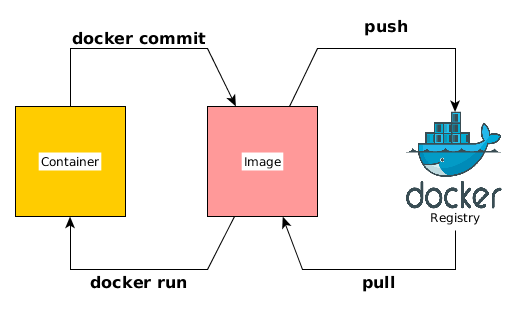
\includegraphics[scale=0.7]{5-patterns/images/docker-registry.png}
 \caption{Docker Registry}
 \label{fig:docker-registry}
 \end{figure}

\end{description}

\section{Event-Driven Messaging}

\begin{description}

\item[Traceability]~\\
The notification mechanism of the Docker Registry uses the Even-Driven Messaging Pattern.

\item[Source]~\\
http://soapatterns.org/designpatterns/eventdrivenmessaging

\item[Issue]~\\ The user wants to be alerted about certain events occuring in his registry.
The notification system needs a mechanism in order to send the events to the user.

\item[Assumptions/Contrainst]~\\ This pattern is used at a lower level in the Docker Registry/Active Repository Pattern.

%\item[Solution]~\\

\item[Rationale]~\\ 

\quote {"Notifications are sent to endpoints via HTTP requests. Each configured endpoint has isolated queues, retry configuration and http targets within each instance of a registry. When an action happens within the registry, it is converted into an event which is dropped into an inmemory queue. When the event reaches the end of the queue, an http request is made to the endpoint until the request succeeds. The events are sent serially to each endpoint but order is not guaranteed."}

\item [Related Patterns]~\\
Active Repository Pattern

%\item [Related Quality Attributes/Key drivers]~\\

\end{description}

\begin{figure}[H]
\centering
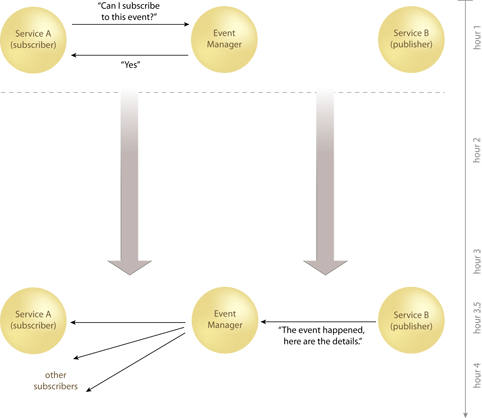
\includegraphics[scale=2]{images/EDM.png}
\caption{Event-Driven Messaging}
\label{fig:event-driven}
\end{figure}

\section{Direct Authentication}
%Brokered Authentication


\begin{description}

\item[Traceability]~\\
The Direct Authentication pattern can be deducted from the source code through the "auth.go" file from the Docker Github Repository. \\
The notification mechanism of the Docker Registry uses this pattern.
\quote{Since securing access to your hosted images is paramount, the Registry natively supports TLS and basic authentication.}

\item[Source]~\\
\textit{https://msdn.microsoft.com/en-us/library/ff647715.aspx} \\
%http://soapatterns.org/design_patterns/direct_authentication
%https://docs.docker.com/registry/spec/auth/token/


\item[Issue]~\\ The Docker Registry needs an authentication system in order to ensure security for the user through a login.

%\item[Assumptions/Contrainst]~\\ 

\item[Solution]~\\ By using the Direct Authentication the access to the Docker Registry is controlled for each user.

\item[Rationale]~\\ 

\item [Related Patterns]~\\
Shared/Active Repository Pattern

\item [Related Quality Attributes/Key drivers]~\\
Security

\end{description}

\section{Plugin}
\label{sec:pattern-plugin}
%TODO image
\begin{description}

\item [Traceability]~\\
The existence of Docker Plugins becomes apparent from its documentation at \cite{dockerplugindocs}.

Additionally, the directories \verb|docker/pkg/plugins/| \footnote{\url{https://github.com/docker/docker/tree/master/pkg/plugins}} and \verb|  docker/daemon/graphdriver/plugin.go| \footnote{\url{https://github.com/docker/docker/blob/master/daemon/graphdriver/plugin.go}} (among others) in the project's repository contain the code for discovering plugins and the interfaces the plugins should implement.

\item [Source]~\\
Patterns of Enterprise Application Architecture, P. 499 \cite{eaa}

\item [Issue]~\\
The users of Docker want to have customization or require functionality that is not included in Docker, by extending Docker with third party custom-built tools. This customization means that third parties should be able to write their own tools that extend Docker's core functionality\cite{dockerpluginblog}.

The implementation of such third party custom-built tools are only available at runtime.

\item [Assumptions/Constraints]~
\begin{itemize}
\item Plugins can only extend the functionality of the components of Docker if they have an interface that plugins can implement.
\end{itemize}

\item [Solution]~\\
Docker uses the Plugin pattern to link the implementation of the interfaces of several extendable components with third-party implementation at runtime.

\item [Rationale] ~\\ % https://docs.docker.com/engine/extend/plugin_api/
Docker discovers plugins by looking for .sock, .spec or .json files in the plugin directories on the host system. These files describe how Docker can communicate with the plugins using the REST API (usually via a Unix socket).

The plugins themselves run as separate processes on the same host as the Docker daemon and implement an HTTP server listening for requests from the Docker daemon. After a user requires a plugin (this is indicated e.g. as a command-line parameter when starting a container using the Docker client) Docker uses the discovery algorithm (see also Section~\ref{sec:processplugins}). After that, Docker sends a handshake to the plugin and the plugin returns a list of which subsystems this plugin implements.

For these subsytems Docker will replace the default implementation by a Proxy, that forwards all calls over the REST interface to the plugin process.

\item [Implications]~\\
The use of the Plugins pattern means that the adaptability increases, because plugins allow the application to be adapted with new features.

For the security, it means that there is extra communication over the API which has to be secured. The security of the plugins themselves cannot be guaranteed by Docker.

\item [Related Patterns]~
\begin{itemize}
\item Proxy
\end{itemize}
\end{description}

\section{Proxy}
\begin{description}

\item [Traceability]~\\
The use of the \pattern{proxy} pattern becomes apparent from the source code in the repository on GitHub.
For example, the proxy for the Volumes plugin can be found in \verb|docker/daemon/graphdriver/proxy.go| \footnote{\url{https://github.com/docker/docker/blob/master/daemon/graphdriver/proxy.go}}.

\item [Source]~\\
Pattern-oriented Software Architecture - Volume 4, P.290 \cite{wiley4}

\item [Issue]~\\
The plugins are separate processes than the daemon and are only available at runtime. Therefore, it is impossible for the daemon process to access the services of the plugins directly.
% issue also for comms between client-server ??

\item [Assumptions/Constraints]~
\begin{itemize}
\item The plugins have to implement a server listening for requests from the daemon.
\end{itemize}

\item [Solution]~\\
Let the daemon only communicate with the plugins through a proxy. This proxy implements all the `housekeeping' functionality, like sending API requests and authentication. It has the same interface as the plugin. \\
Whenever a call is done from the daemon to the plugin, it goes via the proxy, which communicates this call using a REST API to the plugin process.

\item [Rationale] ~\\ 
Using the \pattern{proxy} pattern allows the daemon to communicate with the plugins, without requiring direct access to these plugins. \\
Also, because the subsystem component has the same interface as its proxy, the implementation of software using this component does not depend on whether the proxy is used or the original subsystem. 

\item [Implications]~\\
The use of the \pattern{proxy} pattern allows communication with the plugins, which increases the extendability. 
Because the communication with the process is not direct, there is some performance overhead.
%TODO: what about portability??

\item [Related Patterns]~
\begin{itemize}
\item Plugin
\end{itemize}

\end{description}

